\chapter{State-of-the-Art}
\label{chap:stateofart}
\thispagestyle{plain}

In this chapter, we review the state-of-the-art of the problem at hand. We start by describing why timetabling is a rather complex problem, some possible approaches to solve it and some of the existing solutions, specifically for the \gls{itc2007} benchmarks.\\

\section{Timetabling Problem}

When solving timetabling problems, it is possible to generate one of multiple types of solutions which are: \textit{feasible}, \textit{non feasible}, \textit{optimal} or \textit{sub-optimal}. A feasible solution solves all the mandatory constraints, unlike non feasible solutions. An optimal solution is the best possible feasible solution given the problem constraints. A problem may have multiple optimal solutions. Lastly, sub-optimal solutions are feasible solutions with sub-optimal values.\\
\\
Timetabling automation is a subject that has been a target of research for about 50 years. The timetabling problem may be formulated as a search or an optimization problem \cite{Schaerf1999}. As a search problem, the goal consists on finding a feasible solution that satisfies all the hard constraints, while ignoring the soft constraints. By posing the timetabling problem as an optimization problem, one seeks to minimize the violations of soft constraints while satisfying the hard constraints. Typically, the optimization is done after the use of a search procedure to find an initial feasible solution.\\
\\
The basic examination timetabling problem, where only the \textit{clash} hard constraint is observed, reduces to the well-known graph \gls{gc} \cite{Jensen2001}. The clash hard constraint specifies that no conflicting exams should be scheduled at the same time slot. Deciding whether a solution exists in the \gls{gc} problem, is a NP-complete  problem \cite{Arora2009}~\cite{Qu2009}. Considering the \gls{gc} as an optimization problem, it is proven that the task of finding the optimal solution is also a NP-Hard  problem \cite{Arora2009}~\cite{Qu2009}. \gls{gc} problems are further explained in Section \ref{sec:ExistingAppr}
\\
%%%%%%%%%%%%%%%%%%%%
\section{Existing Approaches}
\label{sec:ExistingAppr}
%%%%%%%%%%%%%%%%%%%%
\begin{figure}[b!]
 \centering
   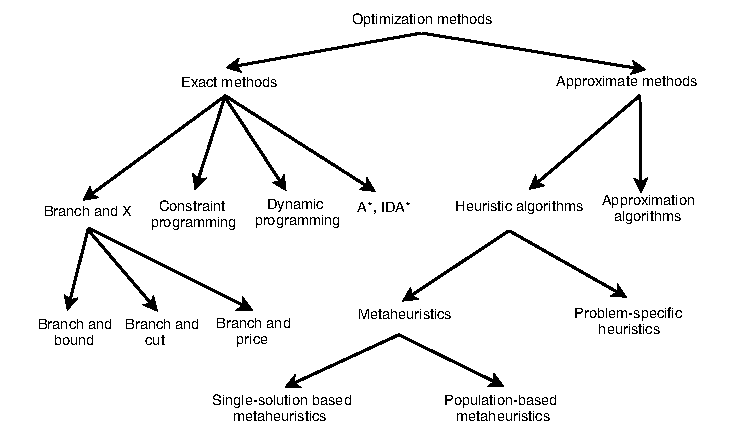
\includegraphics[width=1\textwidth,natwidth=1317,natheight=814]{./images/typesOfAlgorithms.pdf}
   \caption{Optimization methods: taxonomy and organization (adapted from \cite{Talbi2009}).}
   \label{fig:TypesAlgorithms}
\end{figure}

Figure \ref{fig:TypesAlgorithms} depicts a taxonomy for the known optimization methods. These methods are divided into \textit{Exact methods} and \textit{Approximate methods}.\\
\\
Timetabling solution approaches are usually divided into the following categories~\cite{Qu2009}: \textit{exact algorithms} (Branch-and-Bound, Constraint Programming), \textit{graph based sequential techniques}, \textit{Single-solution based meta-heuristics} (Tabu Search, Simulated Annealing, Great Deluge), \textit{population based algorithms} (Evolutionary Algorithms, Memetic algorithms, Ant Colony algorithms, Artificial immune algorithms), \textit{Multi-criteria techniques}, \textit{Hyper-heuristics}, and \textit{Decomposition/clustering techniques}. Hybrid algorithms, which combine features of several algorithms, comprise the state-of-the-art. Due to its complexity, approaching the examination timetabling problem using exact method approaches, can only be done for small size instances. Real problem instances found in practice, are usually of large size, making the use of exact methods impracticable. Heuristic solution algorithms have been usually employed to solve this problem.\\
\\
Real problem instances are usually solved by algorithms which use both \textit{heuristics} and \textit{meta-heuristics}. Heuristic algorithms are problem-dependent, meaning that these are adapted to a specific problem in which one can take advantage of its details. Heuristics are usually applied to obtain a solution, which may be feasible or not. For instance, \gls{gc} heuristics are used to obtain solutions for a given timetable problem instance. Usually only the hard constraints are considered in this phase. Meta-heuristics, on the other hand, are problem-independent, and are used to optimize any type of problem. In these, one usually considers both hard and soft requirements.\\
\\
Most of the existing meta-heuristic algorithms belong to one of the following three categories: One-Stage algorithms, Two-Stage algorithms and algorithms that allow relaxations~\cite{Lewis2007}. The One-Stage algorithm is applied to get a solution, whose goal is to satisfy both hard and soft constraints, at the same time. The Two-Stage algorithms are the most frequent types of approaches. This category is divided in two phases: the first phase consists in not considering the soft constraints and focusing on solving hard constraints to obtain a feasible solution; the second phase is an attempt to find the best solution, trying to solve the largest number of soft constraints as possible, given the solution of the first phase. Algorithms that allow relaxation can weaken some constraints in order to solve the \textit{relaxed problem}, while considering the satisfaction of the original constraints that were weakened, on a later stage of the algorithm.

\subsection{Exact methods}
\label{subsec:ExactMethods}
Approximation algorithms like heuristics and meta-heuristics proceed to enumerate partially the search space and, for that reason, they can't guarantee to find the optimal solution. Exact approaches perform an implicit enumeration of the search space and thus guarantee that the encountered solution is optimal. A negative aspect is the time taken to find the solution. If the decision problem is very difficult (e.g., NP-Complete), in practical scenarios, given the large size problem instances, it may not be possible to use this approach due to the prohibitive time.\\

\subsubsection{Constraint-Programming Based Technique}
The \gls{cpbt} \cite{Boizumault1996} allows direct programming with constraints which gives ease and flexibility in solving problems like timetabling. Two important features of this technique are the use of backtracking and logical variables. Constraint programming is different from other types of programming, in the sense that it specifies the steps that need to be executed, but in constraint programming only the properties (hard constraints) of the solution, or the properties that should not be in the solution, are specified \cite{Qu2009}.\\

\subsubsection{Integer Programming}
The \gls{ip} \cite{Al-Yakoob2010} is a mathematical programming technique in which the optimization problem to be solved must be formulated as an Integer Problem. If both the objective function and the constraints are linear, and all problem variables are integer valued, then the \gls{ip} problem is termed \gls{ilp}. In the presence of both integer and continuous variables, then the problem is called \gls{milp}. Schaerf~\cite{Schaerf1999} surveys some approaches using the \gls{milp} technique to school, course, and examination timetabling.\\

\subsection{Graph Coloring Based Techniques}
\label{subsec:GraphColoring}
As mentioned previously, timetabling problems can be reduced to a \gls{gc} problem. Exploiting the connection between these two problems, several authors used two-phase algorithms in which \gls{gc} heuristics are applied in the first phase, to obtain an initial feasible solution.\\

\subsubsection{Graph Coloring Problem}
The \gls{gc} problem consists in assigning colors to an element type of a graph which must follow certain constraints. The simplest sub-type is the \textit{vertex coloring}, which the main goal is to, given a number of vertices and edges, color the vertices so that no adjacent vertices have the same color. In this case, the goal is to find a solution with the lowest number of colors as possible.\\
\\
The examination timetabling problem can be transformed into a \gls{gc} problem as follows. The exams corresponds to vertices and there exists an edge connecting each pair of conflicting exams (exams that have students in common). With this mapping only the clash hard constraints are taken into consideration. Thus, soft constraints are ignored \cite{Qu2009}.\\
\\
Given the mapping between the \gls{gc} problem and the examination timetabling problem, \gls{gc} heuristics like \textit{Saturation Degree Ordering} are very commonly used to get the initial solutions. Others like \textit{First Fit} and other \textit{Degree Based Ordering} techniques (\textit{Largest Degree Ordering}, \textit{Incidence Degree Ordering}) are also heuristic techniques for coloring graphs~\cite{Carter1996}.

%\paragraph{Saturation Degree Ordering}
%The Saturation Degree Ordering heuristic colors the vertices with more constraints first. The coloring method is as follows: while choosing a vertice to color, the ones with higher saturation degree will be colored first. The saturation degree of one vertice is the number of differently colored vertices adjacent to this vertice or, in another words, the number of different colors of all adjacent vertices. In the case of a tie, the highest saturation vertice with higher number of adjacent vertices is chosen.

\subsection{Meta-heuristics}
\label{subsec:MetaHeuristics}
Meta-heuristics, as mentioned above, usually provide solutions for optimization problems. In timetabling problems, meta-heuristic algorithms are used to optimize the feasible solutions provided by heuristics, such as the \gls{gc} heuristics. Meta-heuristics are divided in two main sub-types, which are \textit{Single-solution meta-heuristics} and \textit{Population-based meta-heuristics}~\cite{Talbi2009}.

\subsubsection{Single-solution meta-heuristics}
Single-solution meta-heuristics main goal is to modify and to optimize one single solution, maintaining the search focused on local regions. This type of meta-heuristic is therefore exploitation oriented. Some examples of this type are \textit{\gls{sa}}, \textit{Variable-Neighborhood Search}, \textit{\gls{ts}}, and \textit{Guided Local Search}~\cite{Talbi2009}. 

\subsubsection{Population-based meta-heuristics}
Population-based meta-heuristics main goal is to modify and to optimize multiple candidate solutions, maintaining the search focused in the whole space. This type of meta-heuristic is therefore exploitation oriented. Some examples of this type are \textit{Particle Swarm}, \textit{Evolutionary Algorithms}, and \textit{Genetic Algorithms}~\cite{Talbi2009}.

\subsection{ITC2007 Examination timetabling problem: some approaches}
\label{subsec:ApprITC2007}

In this section, the five \gls{itc2007} - Examination timetabling track - finalists approaches are described. This timetabling problem comprises 12 instances of different degree of complexity. Through the available website, competitors could submit their solutions for the given benchmark instances. The submitted solutions were evaluated as follows. First, it is checked if the solution is feasible and a so-called distance to the feasibility is computed. If it is feasible, the solution is further evaluated based on the fitness function, which measures the soft constraints total penalty. Then, competitors' solutions are ranked based on the distance to feasibility and solution's fitness value. The method achieving the lower distance to feasibility value is the winner. In the case of a tie, the competitor's solution with the lowest fitness value wins. A solution is considered feasible if the value of distance to feasibility is zero. \\
\\
The set of hard constraints is the following:
\begin{itemize}
	\item no student must be elected to be present in more than one exam at the same time;
	\item the number of students in a class must not exceed the room's capacity;
	\item exam's length must not surpass the length of the assigned time slot;
	\item exams ordering hard constraints must be followed; e.g., $Exam_1$ must be scheduled after $Exam_2$;
	\item room assignments hard constraints must be followed; e.g., 	$Exam_1$ must be scheduled in $Room_1$.
\end{itemize}
It is also necessary to compute the fitness value of the solution which is computed by the average sum of the soft constraints penalty. The soft constraints are listed below:
\begin{itemize}
	\item two exams in a row -- a student should not be assigned to be in two adjacent exams in the same day;
	\item two exams in a day -- a student should not be assigned to be in two non adjacent exams in the same day;
	\item period spread -- the number of times a student is assigned to be in two exams that are \textit{N} time slots apart should be minimized;
	\item mixed durations -- the number of exams with different durations that occur in the same room and period should be minimized;
	\item larger exams constraints - reduce the number of large exams that occur later in the timetable;
	\item room penalty -- avoid assigning exams to rooms with penalty;
	\item period penalty -- avoid assigning exams to periods with penalty.
\end{itemize}
in order to get a detailed description on how to compute the values of fitness and distance to feasibility based on the weight of each constraint, please check the \gls{itc2007} website~\cite{McCollum2007}.\\
\\
We now review the \gls{itc2007}'s five winners approaches. The winners list of the \gls{itc2007} competition is as follows:
\begin{itemize}
	\item 1st Place - Tom\'{a}\v{s} M\"{u}ller
	\item 2nd Place - Christos Gogos
	\item 3rd Place - Mitsunori Atsuta, Koji Nonobe, and Toshihide Ibaraki
	\item 4th Place - Geoffrey De Smet
	\item 5th Place - Nelishia Pillay
\end{itemize}
We now briefly describe these approaches.\\
\\
Tom\'{a}\v{s} M\"{u}ller's approach \cite{Mueller2009} was actually applied to solve the three problems established by the \gls{itc2007} competition. He was able to win two of them and to be finalist on the third. For solving the problems, he opted for an hybrid approach, organized in a two-phase algorithm. In the first phase, Tom\'{a}\v{s} used the Iterative Forward Search (IFS) algorithm \cite{Mueller2005} to obtain feasible solutions and Conflict-based Statistics \cite{Mueller2004} to prevent IFS from looping. The second phase consists in using multiple optimization algorithms. These algorithms are applied in this order: \gls{hc} \cite{Russell2010}, \gls{gd} \cite{Dueck1993}, and optionally \gls{sa}~\cite{Kirkpatrick1983}.\\
\\
Gogos was able to reach second place in the Examination Timetabling track. Gogos' approach~\cite{Gogos2012}, like M\"{u}ller's, is a two-phase approach. The first phase starts with a pre-processing stage, in which the hidden dependencies between exams are checked in order to speed up the optimization phase. After the pre-processing stage, a construction stage takes place, using a meta-heuristic called \textit{\gls{grasp}}. In the second phase, optimization methods are applied in this order: \gls{hc}, \gls{sa}, \gls{ip} (the Branch and Bound procedure), finishing with the so-called Shaking Stage, which is applied only on certain conditions. The Shaking Stage \textit{shakes} the current solution creating an equally good solution, which is given to the \gls{sa}. The objective of this stage to force \gls{sa} to restart with more promising solutions and to generate better results.\\
\\
Atsuta et al. ended up in third place on the Examination Timetabling track and won third and second places on the other tracks, with the same approach for all of them. Their approach \cite{Atsuta2007} consists on applying a constraint satisfaction problem solver adopting an hybridization of \gls{ts} and Iterated Local Search.\\
\\
Geoffrey De Smet's approach \cite{Smet2007} differs from all others because he decided not to use a known problem-specific heuristic to obtain a feasible solution, but instead used what is called the \textit{Drool's rule engine}, named \textit{drools-solver} \cite{Drools}. The drools-solver is a combination of optimization heuristics and meta-heuristics with very efficient score calculation. A solution's score is the sum of the weight of the constraints being broken. After obtaining a feasible solution, Geoffrey opted to use a local search algorithm, namely \gls{ts}, to improve the solutions obtained using the drools-solver.\\
\\
Nelishia Pillay opted to use a two-phase algorithm variant, using a \textit{Developmental Approach based on Cell Biology} \cite{Pillay2007}, whose goal consists in forming a well-developed organism by the process of creating a cell, proceeding with cell division, cell interaction, and cell migration. In this approach, each cell represents a time slot. The first phase represents the process of creating the first cell, cell division, and cell interaction. The second phase represents the cell migration.

\subsection{Other methods - further approaches}
\label{subsec:OtherAppr}

In this subsection, we describe other approaches to the ITC 2007 problem, which were proposed after the 2007 contest.\\
\\
Abdullah et al.'s 2009 approach \cite{Abdullah2009} consists on using an hybridization of an electromagnetic-like mechanism and the \gls{gd} algorithm. In this approach, the electromagnetism-like mechanism starts with a randomly generated population of timetables. Electromagnetic-like mechanism is a meta-heuristic algorithm using an \textit{attraction-repulsion} technique \cite{Javadian2008} to move the solutions to the region of optimal solutions.\\
\\
McCollum et al.'s 2009 two phase approach \cite{McCollum2009} applies an adaptive ordering heuristic from \cite{Burke2004}, proceeding with an \textit{extended version} of \gls{gd}. As the author stated, this approach is robust and generic considering the obtained results on the benchmark datasets from \gls{itc2007}.\\
\\
Alzaqebah et al.'s 2011 two phase approach \cite{Alzaqebah2011} starts by using a \gls{gc} heuristic (largest degree ordering) to generate the initial solution. It ends by applying the \textit{Artificial Bee Colony} search algorithm to optimize the solution.\\
\\
Turabieh and Abdullah's 2011 approach \cite{Turabieh2011} utilizes a two phase algorithm. The first phase consists on constructing initial solutions by using an hybridization of \gls{gc} heuristics (least saturation degree, largest degree first and largest enrollment). The second phase utilizes an hybridization of electromagnetic-like mechanism and \gls{gd} algorithm, just like in \cite{Abdullah2009}.\\
\\
Turabieh and Abdullah proposed another approach in 2012 \cite{Abdullah2012} that utilizes a Tabu-based memetic algorithm which consists on an hybridization of a \gls{ga} with \gls{ts} algorithms. The authors claim that this approach produces some of the best results, when tested on the \gls{itc2007}'s datasets.\\
\\
Demeester et al. in 2012 created an hyper-heuristic approach \cite{Demeester2012}. The heuristics that were considered are 'improved or equal', equivalent to hill climbing that accepts equally good solutions, \gls{sa}, \gls{gd}, and an adapted version of the \textit{late acceptance} strategy \cite{Burke2008}. These heuristics are used on already-created initial solutions. Initial solutions are constructed using an algorithm which does not guarantee the feasibility of the solution.\\
\\
McCollum et al.'s 2012 approach \cite{McCollum2012} introduce an \gls{ip} formulation to the \gls{itc2007} instance, and also a solver using the CPLEX software.\\
\\
Sabar et al.'s utilized a \gls{gc} hyper-heuristic on its approach in 2012 \cite{Sabar2012}. This hyper-heuristic is composed of four hybridizations of these four methods: last degree, saturation degree, largest colored degree and largest enrollment. This approach seems to compete with the winners' approaches from \gls{itc2007}, considering the benchmark results.\\
\\
Sabar et al.'s 2012 approach \cite{Sabar2012a} utilizes a two phase algorithm. It starts by using an hybridization of \gls{gc} heuristics to obtain feasible solutions and a variant of honey-bee algorithm for optimization. The hybridization is composed of least saturation degree, largest degree first, and largest enrollment first, applied in this order.\\
\\
Abdullah and Alzaqebah opted to create an hybridization approach in 2013 \cite{Abdullah2013}, mixing the use of a modified bees algorithm with local search algorithms (i.e. \gls{sa} and late acceptance \gls{hc}).\\
\\
Salwani Abdullah and Malek Alzaqebah in 2014 constructed an approach \cite{Alzaqebah2014} that utilizes an hybridization of a modified artificial bee colony with a local search algorithm (i.e. late acceptance \gls{hc}).\\
\\
Burke et al.'s 2014 approach \cite{Burke2014} uses an hyper-heuristic with hybridization of low level heuristics (neighbor operations) to improve the solutions. The low level heuristics are \textit{move exam}, \textit{swap exam}, \textit{kempe chain move} and \textit{swap times lot}. After applying this hyper-heuristic with the hybridizations, the hybridization with the best results was tested with multiple exam ordering methods, applying another hyper-heuristic with hybridizations. The heuristics applied are \textit{largest degree}, \textit{largest weighted degree}, \textit{saturation degree}, \textit{largest penalty}, and \textit{random ordering}.\\
\\
Hmer and Mouhoub's approach \cite{Mouhoub2014} uses a multi-phase hybridization of meta-heuristics. Works like the two phase algorithm but includes a pre-processing phase before the construction phase. This pre-processing phase is divided in two phases: the propagation of ordering constraints and implicit constraints discovery. The construction phase utilizes a variant of \gls{ts}. The optimization phase uses hybridization of \gls{hc}, \gls{sa}, and an extended version of the \gls{gd} algorithm.\\
\\
Hamilton-Bryce et al. \cite{Hamilton-Bryce2014} in 2014 opted to use a non-stochastic method on their approach \cite{Hamilton-Bryce2014}, when choosing examinations in the neighborhood searching process on the optimization phase. Instead, it uses a technique to make an intelligent selection of examinations using information gathered in the construction phase. This approach is divided into 3 phases. The first phase uses a \textit{Squeaky Wheel} constructor which generates multiple initial timetables and a weighted list for each timetable. Only the best timetable and its weighted list is passed to the second phase. The second phase is the \textit{Directed Selection Optimization} phase which uses the weighted list created in the construction phase to influence the selection of examinations for the neighbor search process. Only the best timetable is passed onto the next phase. The third phase is the \textit{Highest Soft Constraint Optimization} phase, which is similar to the previous phase but a weighted list of values is calculated, based on the solution's individual soft constraints penalty.\\
\\
Rahman et al.'s approach \cite{Rahman2014} is a constructive one. This divides examinations in sets called \textit{easy sets} and \textit{hard sets}. Easy sets contain the examinations that are easy to schedule on a timetable and on the contrary, hard sets contain the ones that are hard to schedule and so are identified as the ones creating infeasibility. This allows to use the examinations present on the hard sets first on future construction attempts. There's also a sub-set within the easy set, called \textit{Boundary Set} which helps on the examinations' ordering and shuffling. Initial examinations' ordering  are accomplished by using \gls{gc} heuristics like largest degree and saturation degree heuristics.\\
\\
Rahman et al.'s approach \cite{Rahman2014a} utilizes adaptive linear combinations of graph coloring heuristics (largest degree and saturation degree) with an heuristic modifier. These adaptive linear combinations allow the attribution of difficulty scores to examinations depending on how hard their scheduling is. The ones with higher score, and so harder to schedule, are scheduled using two strategies: using single or multiple heuristics and with or without heuristic modifier. The authors conclude that multiple heuristics with heuristic modifier offers good quality solutions, and the presented adaptive linear combination is a highly effective method.\\
\\
Table \ref{table:timetable} contains a timeline that represents the previous mentioned approaches chronologically ordered.


\begin{table}
\renewcommand\arraystretch{1.4}\arrayrulecolor{LightSteelBlue3}
\captionsetup{singlelinecheck=false, font=blue, labelfont=sc, labelsep=quad}
\caption{Timeline of existing approaches}\vskip -1.5ex
\scalebox{1}{
\begin{tabular}{@{\,}r <{\hskip 2pt} !{\foo} >{\raggedright\arraybackslash}p{15cm}}
\toprule
\addlinespace[1.5ex]
2007	& Atsuta et al. - Constraint satisfaction problem solver using an hybridization of TS and Iterated Local Search.\\
		& Smet - drool's solver with \gls{ts}.\\
		& Pillay - Two phase approach using Developmental Approach based on Cell Biology (creating the first cell, cell division, cell iteration, and cell migrations).\\
2009 	& M\"{u}ller - Two-phase approach with hybridization, which the first phase includes \gls{ifs} and Conflict-based Statistics, and the second phase is composed of \gls{hc}, \gls{gd}, and \gls{sa}.\\
		& Abdullah et al. - Hybridization of electromagnetic-like mechanism and \gls{gd} algorithm.\\
		& McCollum et al. - Two phase approach, which first phase consists on using adaptive ordering heuristic, and the second phase utilizes an \textit{extended version} of \gls{gd}.\\
2011	& Alzaqebah and Abdullah - Two phase approach, which the first phase uses the largest degree ordering, and the second phase utilizes an Artificial Bee Colony search algorithm.\\
		& Turabeih and Abdullah - Two phase approach, which the first phase utilizes an hybridization of \gls{gc} heuristics, and the second phase uses an hybridization of electromagnetic-like mechanism and \gls{gd} algorithm.\\
2012	& Gogos - Considered a two-phase approach with a pre-processing stage for hidden dependencies. The first phase uses the \textit{greedy randomized adaptive search procedure}, and the second phase is composed of \gls{hc}, \gls{sa}, \gls{ip} with Branch and Bound, finishing with a shaking stage.\\
		& Turabieh and Abdullah - Tabu-based memetic algorithm which is an hybridization of a genetic algorithm with \gls{ts}.\\
		& Demeester et al. - Hyper-heuristic approach of 'improved or equal', \gls{sa}, \gls{gd} and late acceptance strategy applied on already created solutions.\\
		& McCollum et al. - Approach based on \gls{ip} formulation.\\
		& Sabar et al. - \gls{gc} hyper-heuristic approach using last degree, saturation degree, largest colored degree and largest enrollment.\\
		& Sabar et al. - Two phase approach, which the first phase is composed of an hybridization of graph coloring heuristics and the second phase uses an honey-bee algorithm.\\
2013	& Abdullah and Alzaqebah - Hybridization approach with a modified bee algorithm and local search algorithms like SA and late acceptance \gls{hc}.\\
2014	& Abdullah and Alzaqebah - Hybridization approach with a modified artificial bee colony with local search algorithm such as late acceptance \gls{hc}.\\
		& Burke et al. - Uses an hyper-heuristic with hybridization of low level heuristics (neighbor operations), thereafter uses an hyper-heuristic with hybridization of exam ordering methods.\\
		& Hmer and Mouhoub - Multi-phase hybridization of meta-heuristics. A two phase approach with pre-processing phase. First phase uses a variant of TS, and the second phase utilizes an hybridization of \gls{hc}, \gls{sa} and an extended version of the \gls{gd} algorithm.\\
		& Brice et al. - Approach with three phases. First phase uses a Squeaky Wheel constructor, second phase utilizes the weighted list created in the first phase for the neighbor search process, and the third phase uses a weighted list based on the solutions' soft constraints penalty.\\
		& Rahman et al. - Constructive approach that divides examinations into easy and hard sets.\\
		& Rahman et al. - Utilizes adaptive linear combinations of \gls{gc} heuristics, like largest degree and saturation degree, with heuristic modifier.\\
		
\end{tabular}
\label{table:timetable}
}
\end{table}